\part{Philosophie}
\label{ch:philosophy}
\chapter*{Philosophie}

\begin{chapquote}{Lewis Carroll, \textit{Alice im Wunderland}}
Die Maus sah sie etwas neugierig an und schien ihr mit dem einen Auge zu
blinzeln; aber sie sagte nichts.
\end{chapquote}

Jemand der Bitcoin nur oberflächlich betrachtet könnte feststellen, dass es
langsam, verschwenderisch, unnötig redundant und zu paranoid ist. Wenn man
Bitcoin jedoch neugierig betrachtet könnte man feststellen, dass die Dinge nicht
so sind, wie sie auf den ersten Blick erscheinen.

Bitcoin hat die Fähigkeit, deine Annahmen zu nehmen und sie auf den Kopf zu
stellen. Nach einer Weile, gerade als du es dir wieder bequem machen wolltest,
wird Bitcoin wie ein Elefant in einem Porzellanladen durch die Wand schlagen und
deine Annahmen noch einmal zerstören.

\begin{figure}
  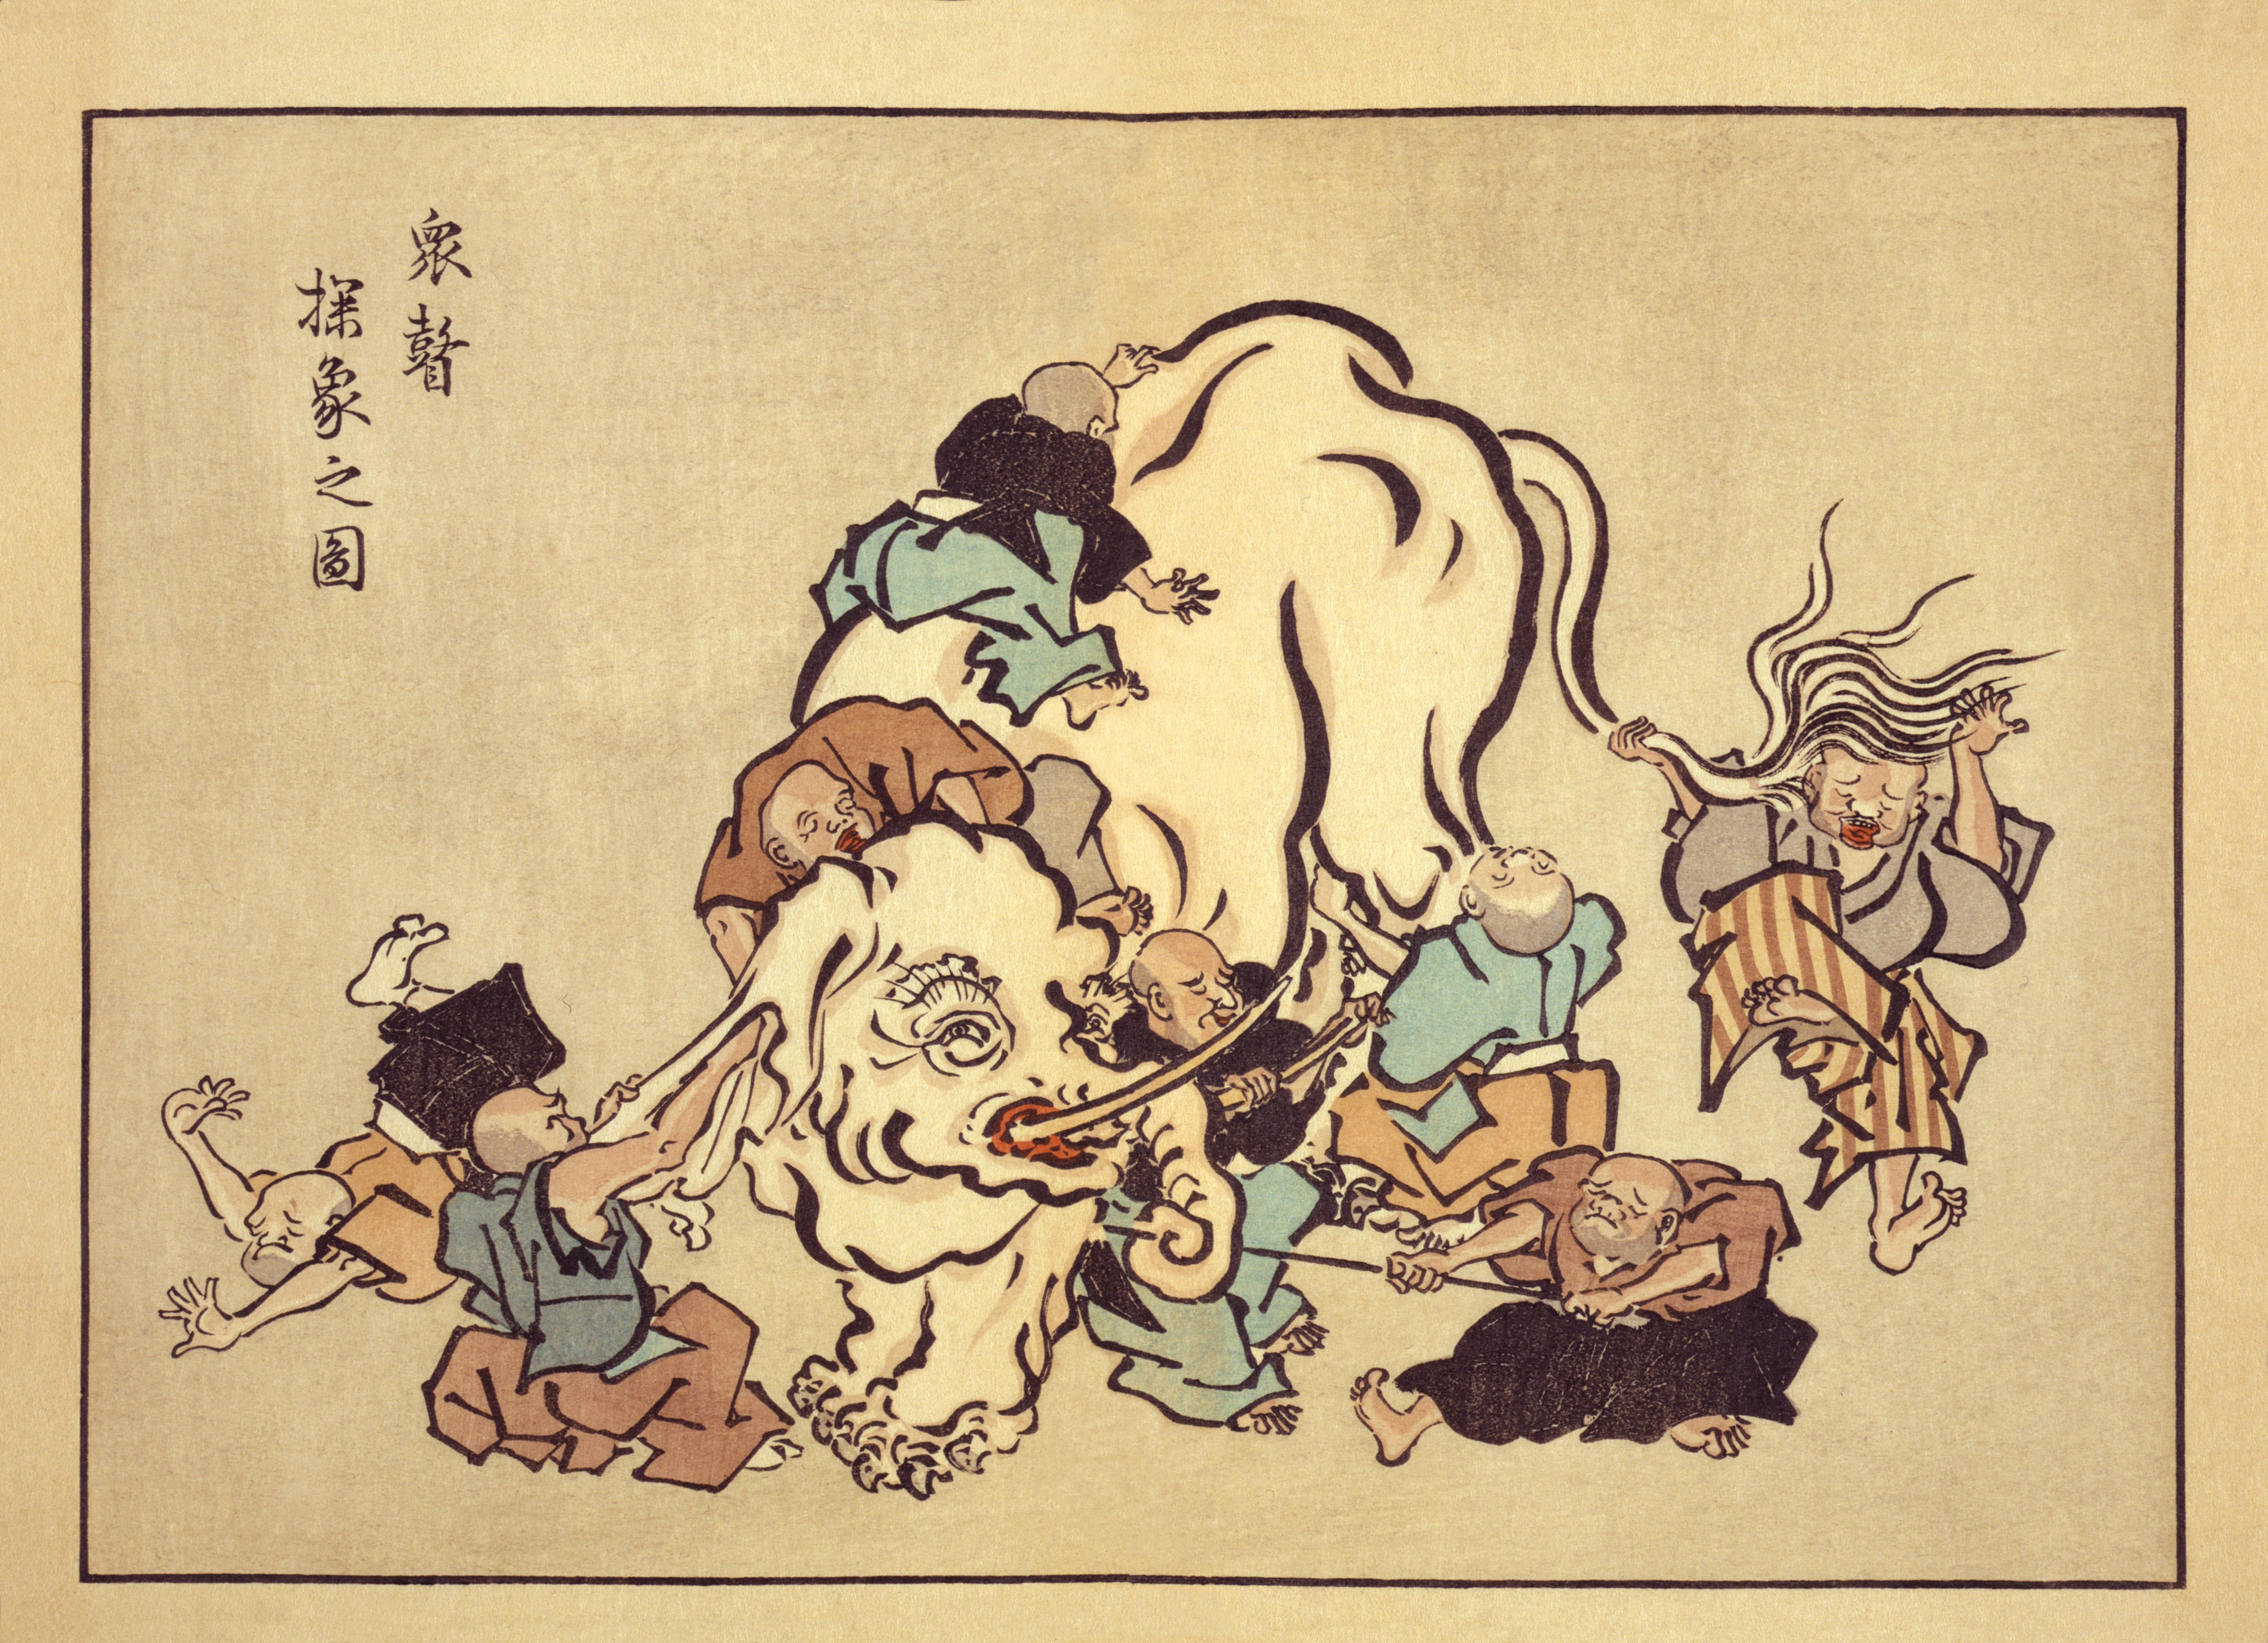
\includegraphics[width=\textwidth]{assets/images/blind-monks.jpg}
  \caption{Blinde Mönche untersuchen den Bitcoin-Elefanten}
  \label{fig:blind-monks}
\end{figure}

Bitcoin ist ein Produkt vieler verschiedener Disziplinen. Wie blinde Mönche, die
einen Elefanten untersuchen, nähern sich dieser neuen Technologie alle aus einem
anderen Blickwinkel. Und jeder wird zu unterschiedlichen Schlussfolgerungen über
die Natur dieses Biests kommen.

Die folgenden Lektionen befassen sich mit einigen meiner Annahmen, die Bitcoin
zunichte gemacht hat, und den Schlussfolgerungen, zu denen ich gekommen bin. In
den ersten vier Lektionen werden philosophische Fragen der Unveränderlichkeit,
der Knappheit, der Lokalität und der Identität untersucht.

~

\begin{samepage}
Teil~\ref{ch:philosophy} -- Philosophie:

\begin{enumerate}
  \item Unveränderlichkeit und Veränderung
  \item Die Knappheit der Knappheit
  \item Replikation und Lokalität
  \item Das Problem der Identität
  \item Eine unbefleckte Empfängnis
  \item Die Macht der freien Meinungsäußerung
  \item Die Grenzen des Wissens
\end{enumerate}
\end{samepage}

Lektion \ref{les:5} untersucht, wie die Entstehungsgeschichte von Bitcoin nicht
nur faszinierend, sondern auch absolut notwendig für ein führerloses System ist.
Die letzten beiden Lektionen dieses Kapitels befassen sich mit der Kraft der
freien Meinungsäußerung und den Grenzen unseres individuellen Wissens, was sich
in der überraschenden Tiefe des Bitcoin Kaninchenbaus zeigt.

Ich hoffe, dass du die Welt von Bitcoin genauso lehrreich, faszinierend und
unterhaltsam finden wirst, wie ich es getan habe und immer noch tue. Ich lade
dich ein, dem weißen Kaninchen zu folgen und die Tiefen dieses Kaninchenbaus zu
erkunden. Jetzt klammer dich an deine Taschenuhr, steige hinab und genieße den
freien Fall.
